\documentclass[a4paper, openany]{memoir}

\usepackage[utf8]{inputenc}
\usepackage[T1]{fontenc} 
\usepackage[english]{babel}
\usepackage{amsmath}
\usepackage{amssymb}

\usepackage{booktabs}
\usepackage{fancyhdr}
\usepackage{float}
\usepackage{indentfirst}
\usepackage{graphicx}
\usepackage[linewidth=1pt]{mdframed}
\usepackage{multicol}
\usepackage{fancyvrb}

\pagestyle{fancy}
\fancyhf{}
\fancyhead[LE]{\leftmark}
\fancyhead[RO]{\rightmark}
\fancyhead[RE, LO]{PSD}
\fancyfoot[LE, RO]{\thepage}
\fancyfoot[RE, LO]{Pete Gautam}

\renewcommand{\headrulewidth}{1.5pt}

\chapterstyle{thatcher}
\setcounter{chapter}{7}

\begin{document}

\chapter{Build, Release and Dependency}
A single software development effort will manage the production of many different labelled releases of the software. Conversely, the software that the team develops will itself depend on versions of the software from other development efforts. 

The team will need to maintain the specification of these dependencies. This allows the dependencies to be retrieved and integrated into the project during a build process. In turn, the releases that the team depends on will report their own dependencies that will also need to be integrated. This eventually produces an assembly of dependencies.

In principle, whenever a team needs a copy of a version of a project, they can clone the required commit from that project's version control repository. However, this would mean that the team would need to clone and package each and every project they depend on, as well as any of their dependencies. This process is typically slow and perhaps not completely automatable.

Build, release and dependency management provides a rigorous means for one software team to build and publish a particular package version to a cache, called the release repository. In turn, other teams can specify their project's dependencies by referencing compiled releases in this cached repository instead of having to specify the source in the version controlled repository. So, build, release and dependency management are distinct, but closely interconnected activities.

\section{Build management}
Almost every programming language environment has an associated build management tool. Modern build management tools also usually integrate dependencies and release managements. Some tools are given below:
\begin{itemize}
    \item Make/configure (C)
    \item Maven (Java)
    \item Ant + Ivy (Java)
    \item Cake (C\#, .net)
    \item Gradle
    \item NPM (Javascript)
    \item setuptools including pip (Python)
    \item Rake (Ruby)
    \item Yum, apt, pkg
    \item Gradle
    \item NuGet
    \item golang/dep.
\end{itemize}

A software project should have a build configuration file. This will contain a mixture of declarative and imperative statements. These describe the targets, mappings and tasks within the build management lifecycle.

Targets are the abstract goals within a software build management lifecycle. They describe the state that a software project's working copy should be left in following the completion of that target. For example, targets might include: 
\begin{itemize}
    \item resolving dependencies,
    \item compiling the code to produce binaries,
    \item testing binaries to produce a report.
\end{itemize}
One target in a software project build lifecycle may depend on other targets. For example, test may first depend on the code being successfully compiled. 

Mappings describe the relationship between source and generated artifacts to be created to reach the target. For example, consider the following mappings.
\begin{figure}[H]
    \centering
    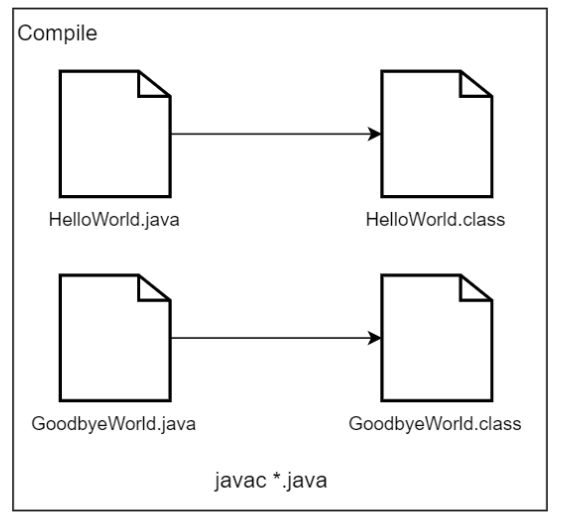
\includegraphics[scale=0.5]{src/8.1 Build Java Example.PNG}
\end{figure}
\noindent The image illustrates the mapping between the source code \texttt{HelloWorld.java} and \texttt{HelloWorld.class}. Mappings are useful for optimising the build process. This is because we can avoid unnecessary tasks that have already been completed. For example, if the \texttt{HelloWorldjava} file has not been altered since \texttt{HelloWorld.class} was compiled, we can avoid the compilation step.

Finally, tasks are the actions that the build management system will take to satisfy mappings. For example, a particular compiler might be executed, or a test suite framework might be executed on a working copy.

There is a many-to-many relationship between the binaries and their target sources. For example, a source file may be involved in the generation of many different types of artifacts. Similarly, a single artifact might be dependent on the availability of several different source resources.

The build process should be repeatable, i.e. the mapping should be idempotent. That is, if we were to repeatedly apply the build process to a given commit, the generated artifact should not change after the first time. For example, when we execute a compile step/target on a project, it should generate a compiled class. Moreover, if the function is operated again, this should not change the state of the compiled files.

Now, consider the following build configuration in MakeFile:
\begin{verbatim}
compile: HelloWorld.class GoodbyeWorld.class

HelloWorld.class: HelloWorld.java
        javac *.java
        
GoodbyeWorld.class: GoodbyeWorld.java
        javac *.java
\end{verbatim}
The build tool has abstract targets (such as \texttt{compile}) and concrete targets (such as \texttt{HelloWorld.class}). It also has mappings from targets (such as \texttt{HelloWorld.class}) to source files (such as \texttt{HelloWorld.java}). It specifies tasks for the completion of the targets, which in this case is the compilation of the files (\texttt{javac *.java}).

\subsection{Targets}
There are many different arrangement for targets within the build management infrastructure. They generally follow a similar pattern to the one given below:
\begin{figure}[H]
    \centering
    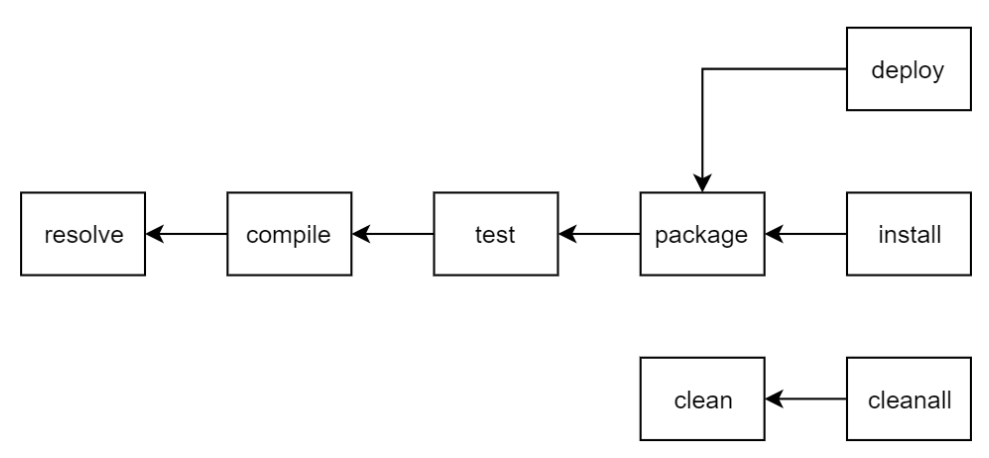
\includegraphics[scale=0.45]{src/8.2 Build Lifecycle.PNG}
    \caption{A typical build lifecycle}
\end{figure}
\noindent We typically start the build lifecycle by a resolve target. This involves collecting dependencies for a software project. This is followed by the compilation target. Here, the source code files are compiled into binaries. Then, we have the test phase. Here, a series of unit (and integration) tests are executed against the compiled code. Finally, we package the compiled binaries into a format suitable for distribution.

There are 2 further processes that might also depend on packaging. We might install the package in the local system's infrastructure. We could also deploy the package to a remote release repository.

Also, supplementary targets (clean and cleanall) are often included in the build management scripts. The clean target removes generated byproducts of the build management process. The cleanall target removes all artifacts generated. The project returns to a pristine state which only has the configuration files.

\subsection{Configuration by convention}
We saw how the Make build management infrastructure requires a very explicit approach to specifying the target's tasks and mapping of a software project. This can lead to very lengthy build configuration scripts which are costly to maintain. 

Modern build management tools often adopt the very useful concept of configuration by convention. This means that the developer should follow most of the conventions set out by the build release tool for the organisation of the software project.

Configuration by convention has many benefits. It minimises the amount of configuration code a project needs to maintain. This is because the associated tooling expects the project to be laid out in a certain way for resource discovery. It facilitates readability by other users and developers of the software project. This is because the convention establishes standard project layouts for the infrastructure. 

% Configuration by convention goes well beyond build management. It can be used for other software frameworks such as web applications.

The following is an example of creating a configuration (by convention) file in the Maven build management infrastructure.
\begin{verbatim}
mvn -B archetype:generate 
    -DgroupId=uk.ac.glasgow.demo 
    -DartifactId=demo-app
\end{verbatim}
This results in the following directory structure:
\begin{verbatim}
|--- pom.xml
|--- src
    |--- main
       |--- uk
           |--- ac
               |--- glasgow
                   |--- demo
                       |--- demo-app
                           |--- App.java
    |--- test
        |--- uk
            |--- ac
                |--- glasgow
                    |--- demo
                          |--- demo-app
                             |--- AppTest.java
\end{verbatim}
In Maven, the project is to be specified by the file \texttt{pom.xml}. There is a single top-level \texttt{src} directory which contains 2 subdirectories.
\begin{itemize}
    \item The \texttt{main} directory contains application code. The package structure of main matches the expected package structure of the group id of the project provided above.
    \item The \texttt{test} directory has an equivalent directory structure. It is responsible for holding unit test code for the project.
\end{itemize}

The file \texttt{pom.xml} has the following data:
\begin{verbatim}
<project>
  <modelVersion>4.0.0</modelVersion>
  <groupId>uk.ac.glasgow.demo</groupId>
  <artifactId>demo-app</artifactId>
  <packaging>jar</packaging>
  <version>1.0-SNAPSHOT</version>
  <name>demo-app</name>
  <dependencies>
    <dependency>
      <groupId>junit</groupId>
      <artifactId>junit</artifactId>
      <version>3.8.1</version>
      <scope>test</scope>
    </dependency>
  </dependencies>
</project>
\end{verbatim}
The document has a number of declarations about the project, such as groupId and artifactID. It also has dependencies. By default, the dependency \texttt{junit} is added.

The layout of the Maven project is declarative. In Maven, we don't specify how tasks are executed. We just declare the high-level naming for the project and leave the details of the actual compilation, testing and packaging to the conventions of the Maven infrastructure.

Configuration by convention does not mean that we must follow the process strictly. It is possible to specify exceptions to the Maven conventions if desired.

\section{Dependency and Release Mangement}
Most software projects exist at a complex graph of dependencies on releases from other software projects, as shown below.
\begin{figure}[H]
    \centering
    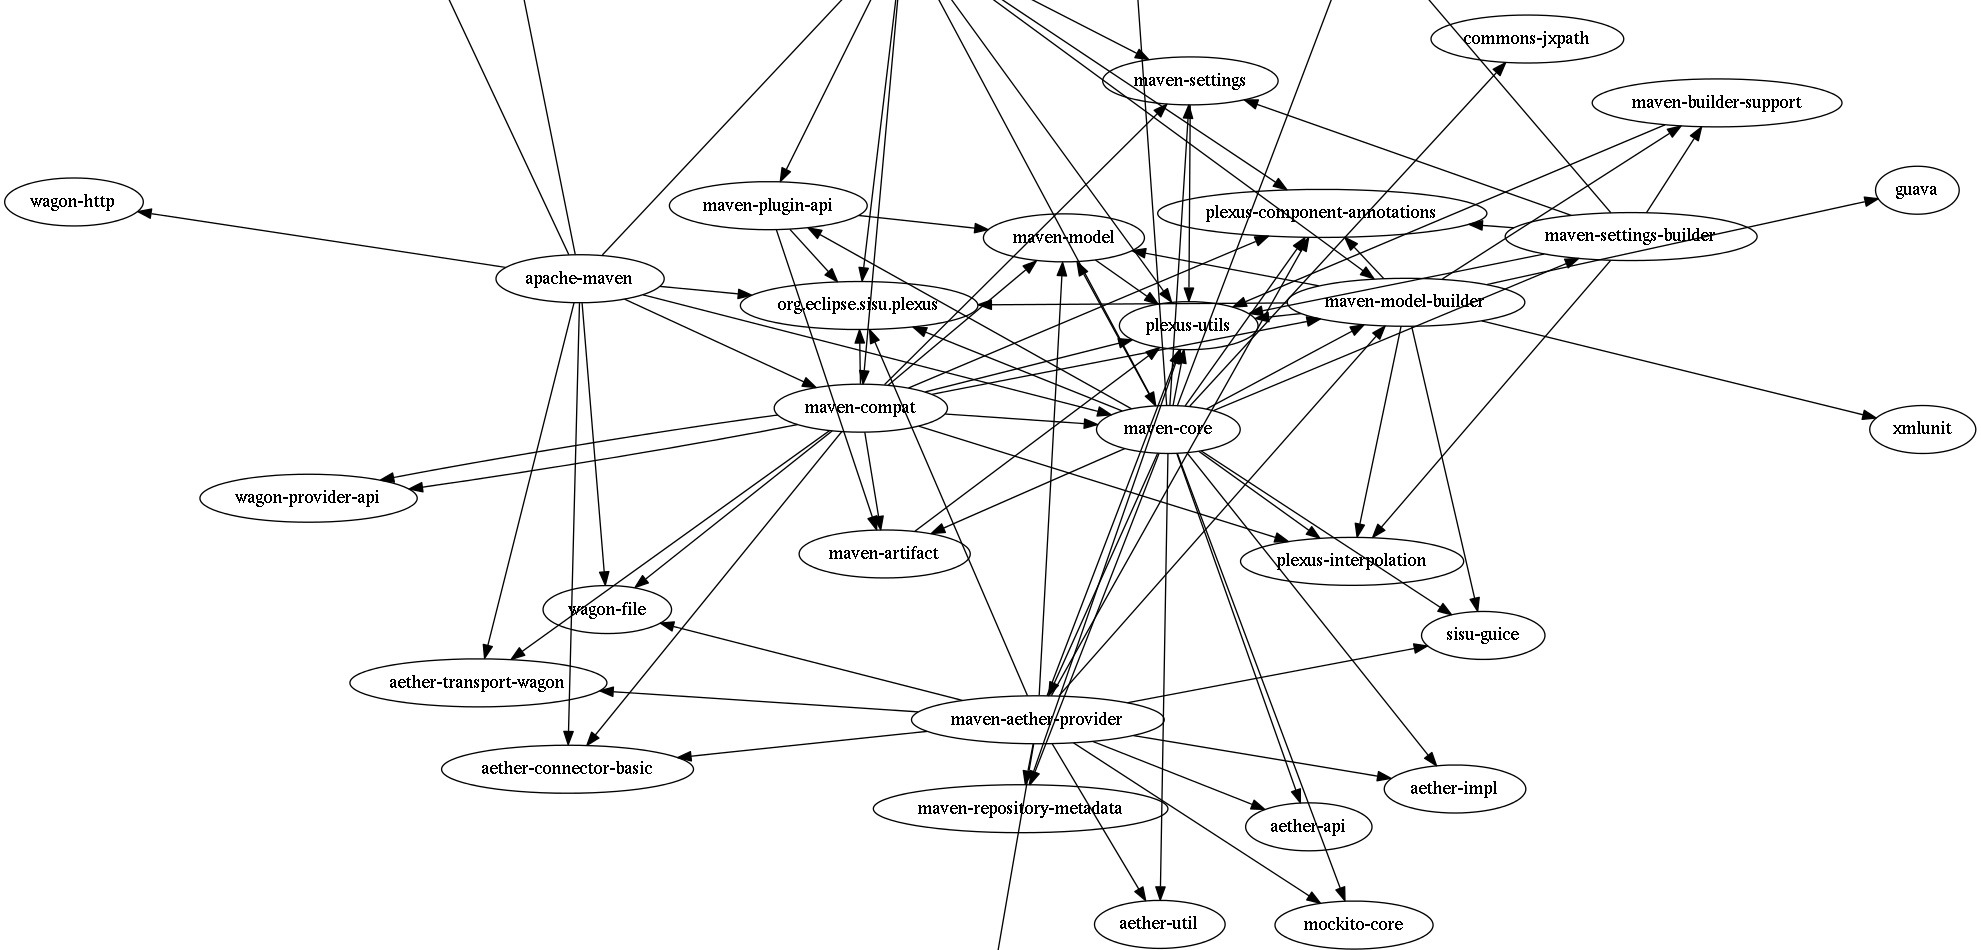
\includegraphics[scale=0.22]{src/8.3 Dependency Graph.png}
\end{figure}
\noindent The diagram illustrates part of the dependency graph of the Maven project. Dependency and release management helps to partially automate the mediation of these graphs. There are 2 types of dependencies- environmental and application dependencies.

Environmental dependencies describe those conditions that must exist in the surrounding infrastructure in order for a particular software system to work. Explicit environmental dependency is when the configuration script lists the dependency. Implicit environmental dependency is when the dependency is assumed to exist and is not explicitly documented within the configuration script. For example, a particular version of the Java SDK is an explicit dependency, while the existence of the Java SDK is an implicit dependency.

Application dependencies describe dependencies on other software components within the build management infrastructure, e.g. a Java library or a Java file.

There are also different types of repositories in a dependency/release management system. A public release repository is better for distributions to customers and for obtaining standard releases of third party libraries. A local release repository can be very useful within the internal network of an organisation for maintaining pre/public stable versions of the components or hard-to-compile components such as datasets. They are also useful for storing specialised internal versions of third party components that have been adapted for an organisational need.

A dependency and release management system will interact with these repositories to follow a workflow comprising of the following tasks:
\begin{itemize}
    \item We first establish requirements of the dependencies for the system;
    \item We obtain a list of available releases for each dependency from the repositories that it knows about.
    \item We choose and check the feasibility of release version combinations from the list of available dependencies. 
    \item We retrieve any missing artifacts from the original release repository.
\end{itemize}

\subsection{Versioning}
It can be very useful to have a labelling scheme to describe and distinguish between different releases of a software component or project. This specification of release versions can be included in a dependency specification for another project in order to select a particular version for integration of the project.

Each release label should be a reference to a particular commit in the version control repository for the project. A release label may also incorporate further information about the release, such as the following.
\begin{itemize}
    \item It may provide temporal relationship to previous and future releases.
    \item It may provide indication about the contents of the release, such as source files, compiled binary, datasets and documentation.
    \item It may provide the purpose of the release, e.g. if it is a production or a snapshot release.
\end{itemize}

\subsection{Specifying dependencies}
A project almost always has transitive dependencies. That is, a project has a dependency on other software projects, and these projects also have dependencies. 

Moreover, dependency graphs may also be cyclic. That is, a project may depend on another project which depends on another project and so on, and we can find a chain of dependencies that ends with the original project. This complicates dependency resolution. In fact, dependency resolution is known to be NP-complete.

Different strategies can be employed to find a satisfactory combination of dependencies. For example, the nearest/first discovered version of the software might be included in assembly. Also, the configuration tool might allow multiple releases to be used in the same assembly and restrict their access to the relevant dependents.

Dependency resolution optimisations mean that ensuring successful dependency is a form of art. If the specifications are under-constrained, we might have a incomplete combination. We might accidentally allow a particular dependency in the project which contains an incompatible API, for example. Instead, if the specifications are over-constrained, we might limit flexibility. It might take more effort to maintain the project. We might persist the use of older, buggier releases if we do not continually update the configuration scripts.

We should migrate to new releases whenever available. This minimises the risk of having vulnerable code integrated to the software system. We should not rely on transitive dependencies. In particular, if we rely on a library transitively, we should include it explicitly in the configuration script.

\subsection{Types of releases}
A release may consist of many types, both in terms of composition and schedule (or intent). The composition might be:
\begin{itemize}
    \item just the core executable binaries;
    \item tailored executable (i.e. one that has been adjusted for particular environment/platform);
    \item optional extensions to the core executable (i.e. additional features that the customer has requested);
    \item other types of releases: package source files for the project, package documentation for executable; the dataset associated with the project; or all of the core executable binaries for the software project, all the dependencies and optional extensions, the source code and documentation in a complete release.
\end{itemize}

A software project release may also have different schedules. Schedules include:
\begin{itemize}
    \item bleeding edge/snapshot, which is a release for each commit of the project.
    \item incremental.
    \item nightly builds, which is typically a release so that integration tests can be executed on them. These tests are too slow to run on every commit.
    \item beta test releases, where packages can be produced for distribution to trusted third parties who can undertake user acceptance tests prior to release.
    \item release candidates, which are a special kind of beta tests that have the potential to be considered the final version of a release.
    \item product release, which is a general release package delivered to end users or customers.
\end{itemize}
Multiple different scheduling schemes may be used in a single project.

\section{Release branching}
In release branching, the team creates a new branch in their version control repository for each release of the software project, as shown in the diagram below.
\begin{figure}[H]
    \centering
    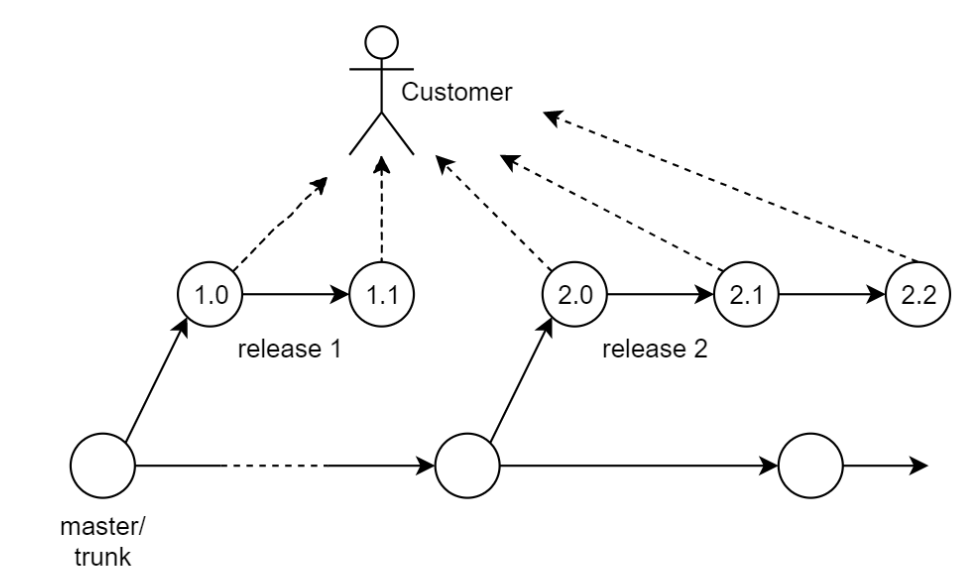
\includegraphics[scale=0.45]{src/8.4 Release Branches.PNG}
\end{figure}
\noindent In the diagram, we have a trunk branch. Periodically, a new branch is created for the release of a software project. Those releases are available to the customer. 

Release branching allows the development team to prepare a new stable release to a customer. In release branches, we only incorporate changes that support bug fixes. These bug fixes can also be merged into master, where new features continue to be developed.

\section{Changes to API}
When preparing a new release of a software system, it is important for the team to consider what changes they have made to APIs within the software system and what impact this might have on dependents. The level of visibility of an API determines how the change to the API should be documented and communicated.

Private APIs are externally inaccessible interfaces. So, documentation for changes to a private API can be minimal, if present at all. Changes to the private API should not have any impact on the dependent because they do not have access to it.

Published features refer to the externally accessible API that the software team has documented as being the expected means of interacting with the system. In this case, the team should document how the change affects users. They should also tell the users how to migrate to the new version. This can either be through some documentation or an automated script.

Public APIs are a superset of published API. These APIs can be externally accessed, but are not necessarily documented as being part of the published API. This can cause some confusion because many languages lack a means of distinguishing between public and published interfaces.

When using such languages, the developers need to maintain support for all public interfaces, whether they expect them to be treated as published or not. Also, some practitioners argue that any externally observable behaviour should be assumed to be at the published level.

For example, a dependent may expect a particular String format for a return value of a toString method in Java. However, the format is an implementation detail, and it is difficult to specify in the language. However, the dependent expects that format to not change. 

To try to counter public APIs, some middleware frameworks provide a means for specifying interfaces at a package level. An example of such a framework is OSGI. This restricts access to any methods within the package and the underlying component unless it is part of the specification.

\subsection{Semantic versioning}
One approach to communicating change is called semantic versioning. In semantic versioning, the version label for a label is formatted as follows:
\[\texttt{major.minor.incremental[-tag]}.\]
An example of this is \texttt{4.0.3-SNAPSHOT}. Going from one release to next, the release number that changes gives an indication of how the change will affect its dependents.
\begin{itemize}
    \item An increase in the incremental (or patch) number denotes a non-breaking change that fixes bugs.
    \item An increase in the minor number denotes a non-breaking change that adds new features.
    \item An increase in the major number denotes a breaking change to the published API. Changes to the software project will be expected to have some impact on dependents.
\end{itemize}
The tag denotes the release status, type or other information about the release.

\subsection{Deprecation}
One approach to mitigate the impact of breaking changes is the use of deprecated features. A deprecated feature is one that has been left in place for compatibility reasons, but will be removed from a future release of the wider system. This motivates the developers to change how they interact with the dependency.

An example of deprecation in Java is given below.
\begin{verbatim}
public abstract class AbstractFactory {
    /**
     * @Deprecated As of release 2.0, replaced by
     * {link #createProduct(String)}. To be removed in 
     * release 3.0.
     */
    @Deprecated public abstract Product createProduct();

    /**
     * @param type if null then the default product is returned.
     */
    public abstract Product createProduct(String type);
}
\end{verbatim}
The older method \texttt{createProduct} has been marked as deprecated. The compiler would generate warnings when using this method, but the process would succeed. The documentation also tells us when the deprecation occurred and how the method has been replaced, and when the old method will be removed from the API.

In general, when documenting a deprecated feature, it is good practice to include:
\begin{itemize}
    \item the scope of the deprecation.
    \item the release version of the software containing the new mechanism.
    \item a schedule for when the deprecated feature will be removed.
    \item an explanation of why the feature has been deprecated.
    \item a description of how to change the dependent code.
\end{itemize}
In some cases, it may also be possible to provide an automated migration script for this purpose.

\subsection{Migration plans and scripts}
When major changes are prepared and published in a release, it is often useful to prepare a migration plan and automation script for dependent. This should explain how to make use of the new release. The migration plan should include:
\begin{itemize}
    \item a means of estimating how long the migration will take.
    \item a summary of known issues with the new release of the software.
    \item data migration, including necessary backups and alterations to data formats (if the software is used in deployed systems).
    \item upgrades of any dependencies of the change software.
    \item how to adapt existing source code to use the new published APIs.
\end{itemize}

In summary, build, release and dependency managements are interdependent workflows that ease the process of inter-component change management by allowing changes to be collated and cached.



\end{document}